Таким образом, постановка изучает оптимизацию как в локальном, так  глобальном поведением агента. Для вычисления исхода конкуренции используем подход, описанный в \cite{Bogdanov2023} для модели Бэрона-Фереджона. В этом случае определяющим свойством игрока является его очередь в формирование предложения. Введем обозначения $R$ для  выигрыша игрока, ходившего первым, и  $r$ - для второго.

Для определения оптимальный величины скидки первый игрок, рассчитает издержки неуспеха для  второго игрока состоящие из издержек в ожидание нового аукциона $P_\text{global}$ и еще один шаг торга $P_\text{local}= i \cdot \text{FC}$.

\begin{figure}[h]
    \centering
    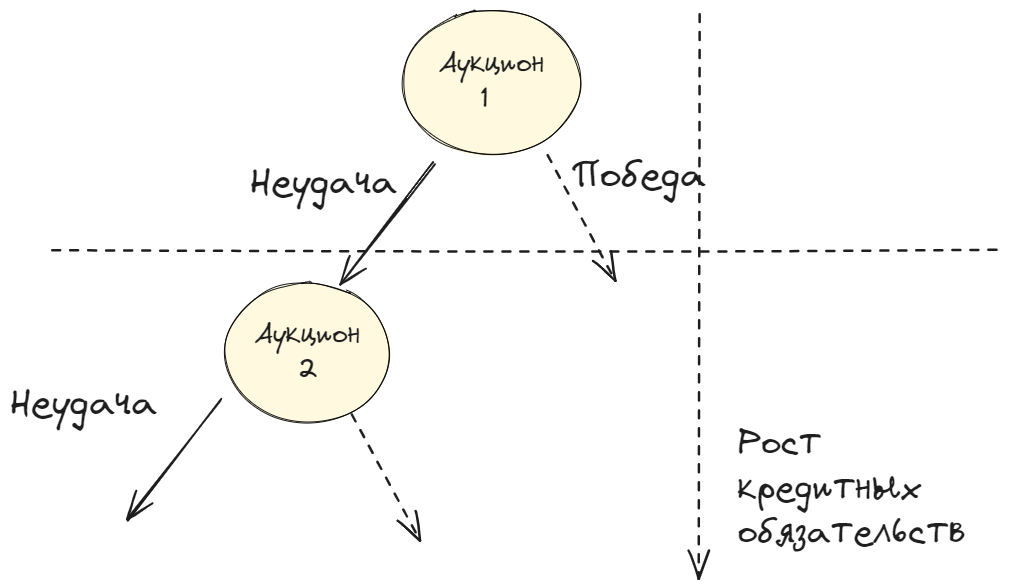
\includegraphics[width=0.5\textwidth]{assets/settings/dynamic.excalidraw.png}
    \caption{Агент при принятии решения учитывает возможность проигрыша в ряде раундов}
\end{figure}

Для определения $P_global$ запишем матожидание по исходам в явной форме:
\begin{equation}
    r  = - FC \cdotp i \cdotp \eta  + 1/ 2 R  + 1/2 \ \cdotp (- FC \cdotp i \cdotp \eta  + 1/2 \ \cdotp (\dots))
\end{equation}

Телескопическая сумма может быть переписана как:
\begin{equation}
    r = R (1/2 + 1/4 + \dots)  - FC \cdotp \ i \ \cdotp (1 +1/2 +1/4 + \dots)    
\end{equation}
    

Сокращая сумму в геометрическую прогрессию получим 
\begin{equation}
    P_{global}= R-r = 2 \ \cdotp FC \ \cdotp \ i \cdotp \ \eta
\end{equation}

Тогда предложение первого поставщика будет определяться как минимум из максимальной скидки $\Delta M_{max} = K_0-FC $ и суммы локальных и глобальных издержек:
\begin{equation}
    \Delta M = \max(\Delta M_{max} - (P_{global} + P_{local}),0) = \max(K_0 - FC \cdotp \ i \ (2 \eta + 1),0)
\end{equation}

Ключевым для заключения сделки является право первого хода. Кредитование пропорционально увеличивает стоимость поставки на величину ликвидности $\eta$ и ставки рефинансирования $i$.
